% ### Uses XeLaTeX ### %
% ### Needs beamer-master ### %
\documentclass[aspectratio=169]{beamer} %. Aspect Ratio 16:9
\usetheme{AI2} % beamerthemeSprace.sty
% DATA FOR FOOTER
\date{2020}
\title{}
\author{}
\institute{Advanced Institute for Artificial Intelligence (AI2)}

\usetikzlibrary{calc,chains,shadows}
\usepackage{tikz}
\usepackage{subfigure}

\begin{document}    
% ####################################
% FIRST SLIDE 						:: \SliTit{<Title of the Talk>}{<Author Name>}{<Intitution>}
% SLIDE SUB-TITLE					:: \SliSubTit{<Title of the Chapter>}{<Title of the Section>}
% SLIDE WITH TITLE 					:: \SliT{<Title>}{Content}
% SLIDE NO TITLE 						:: \Sli{<Content>} 
% SLIDE DOUBLE COLUMN WITH TITLE 	:: \SliDT{<Title>}{<First Column>}{<Second Column>}
% SLIDE DOUBLE COLUMN NO TITLE 		:: \SliD{<First Column>}{<Second Column>}
% SLIDE ADVANCED WITH TITLE 			:: \SliAdvT{<Title>}{<Content>}
% SLIDE ADVANCED  NO TITLE 			:: \SliAdv{<Content>}
% SLIDE ADVANCED DOUBLE TITLE 		:: SliAdvDT{<Title>}{<First Column>}{<Second Column>}
% SLIDE ADVANCED DOUBLE NO TITLE 	:: SliAdvD{<First Column>}{<Second Column>}
% ITEMIZE 							:: \begin{itemize}  \IteOne{1st Level} \IteTwo {2nd Level} \IteThr{3rd Level} \end{itemize}
% SECTION 							:: \secx{Section} | \secxx{Sub-Section}
% COLOR BOX 						:: \blu{blue} + \red{red} + \yel{yellow} + \gre{green}
% FRAME 							:: \fra{sprace} \frab{blue} \frar{red} + \fray{yellow} + \frag{green}	
% REFERENCE						:: \refer{<doi number>}
% FIGURE 							::  \img{X}{Y}{<scale>}{Figures/.png} 
% FIGURE							:: \begin{center}\includegraphics[scale=<#>]{Figures/.png}\end{center}
% PROJECT STATUS					:: \planned\~    \started\~   \underway\~   \done\~   
% EXERCICIO							:: \Exe{<#>}{<text>}
% STACKREL							:: \underset{<down>}{<up>}
% FLUSH LEFT						:: \begin{flalign*}  & <1st equation> & \\  & <12nd equation>  & \\ \end{flalign*}
% REAL / IMAGINAY					:: \Re / \Im
% SLASH								:: \sl{} or \sl
% BOLD MATH							:: \pmb{<>}
% ####################################
%
% FIRST SLIDE :: DO NOT BREAK LINE !!!
\SliTit{Classificação}{Advanced Institute for Artificial Intelligence}{https://advancedinstitute.ai}

\SliT{Classificação}{

Agenda

\begin{itemize}
    \item Curva ROC
    \item Regressão Logística
    \item Naive Bayes
    \item Paradigma de classificação
    \item Transformando classificador binário em classificador multiclasse
    \item KNN
    \item Arvore de Decisão
    
\end{itemize}

}

\SliT{Classificação}{
Curva ROC (\textit{Receiver Operator Characteristic})

\begin{itemize}
\item A relação entre sensibilidade e especificidade pode ser ilustrada usando-se um gráfico conhecido como curva ROC. 

\item Uma curva ROC é um gráfico de linha que mostra a probabilidade de um resultado positivo verdadeiro comparado a probabilidade de um resultado falso positivo para uma série.

\end{itemize}

}

\SliT{Classificação}{
Scikit prove um método para  curva Roc
from sklearn.metrics import roc\_auc\_score

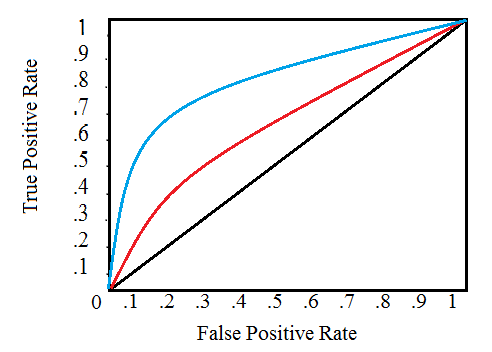
\includegraphics[width=0.55\columnwidth]{ROC-curve.png}

}


\SliT{Classificação}{


\begin{itemize}
\item A regressão logística binária é um tipo de análise de regressão em que a variável dependente é uma variável qualitativa: 0 ou 1

\item Uma função gerada por uma regressão linear considerando uma variável qualitativa 0 ou 1, gera valores fora do intervalo 0 ou 1
\end{itemize}

}
\Sli{
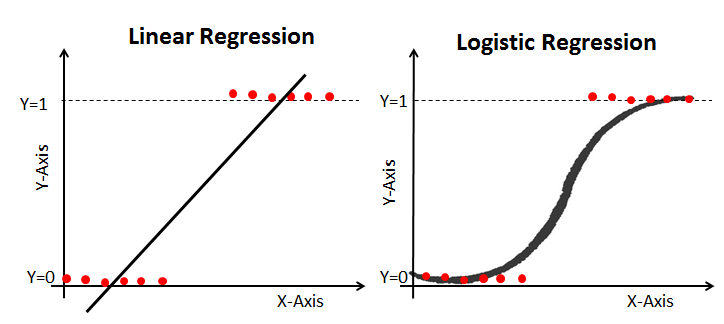
\includegraphics[width=0.85\columnwidth]{12.png}
}

\SliT{Classificação}{

Regressão logística
\begin{itemize}

\item Modelar a probabilidade de um evento ocorrer dependendo dos valores das variáveis independentes.

\item Estimar a probabilidade de um evento ocorrer (e também de não ocorrer) para uma dada observação
\item Distribuição discreta de espaço amostral  {0,1}  que tem probabilidade de sucesso  p  e  falha  q = 1 - p
\end{itemize}

}

\SliT{Classificação}{

Regressão logística

\begin{itemize}

\item Na regressão logística estimamos  p  para qualquer combinação linear das variáveis independentes.

\item Isso pode ser alcançado usando o MLE (\textit{Maximum Likehood Estimation}) para estimar os coeficiente do modelo.

\item Também pode ser usado descida do gradiente, otimizando os coeficientes para aproximar os valores mais próximos de 0 e 1.
\end{itemize}

}

\SliT{Classificação}{

Naive Bayes

\begin{itemize}
\item Baseado na suposição de que as quantidades de interesse são reguladas por distribuições de probabilidades.
\item Quantificar o custo/benefício entre diferentes decisões de classificação usando probabilidades e custos associados à classificação.
\item Teorema de Bayes Mostra como alterar as probabilidades \textit{a priori} tendo em conta novas evidências de forma a obter probabilidades \textit{a posteriori}
\end{itemize}
}

\SliT{Classificação}{

\begin{itemize}
\item Classe $W_1$

\item Probabilidades a priori $P(W_1)$: Conhecimento a priori que se tem sobre o problema, ou seja, conhecimento a priori sobre a aparição de exemplos das classes do problema.
\item Função de Densidade Probabilidade $P(x)$: Frequência com a qual encontramos uma determinada característica (Evidências)
\end{itemize}
}

\SliT{Classificação}{

\begin{itemize}

\item Densidade de Probabilidade Condicional
\item $P(X|W_j)$ (Likelihood) - Verossimilhança
\item Frequência com que encontramos uma determinada característica x dado que a mesma pertence a classe $W_j$
\item Densidade de duas classes em que $x$ representa uma característica qualquer
\end{itemize}
}

\Sli{
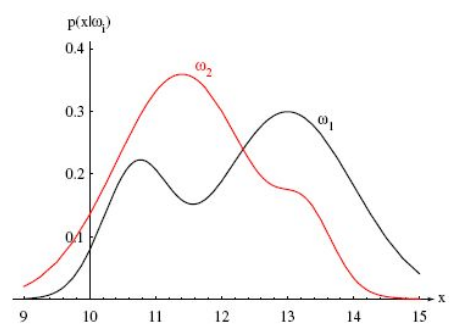
\includegraphics[width=0.65\columnwidth]{1212.png}
}

\Sli{
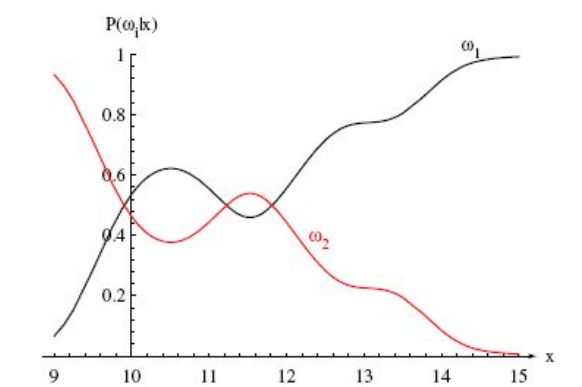
\includegraphics[width=0.65\columnwidth]{1213.png}
}

\SliT{Classificação}{

\begin{itemize}

\item Probabilidades a posteriori para um valor de $x=14$, 
\item a probabilidade do padrão pertencer a $W_1$ é de 0,08, 
\item a probabilidade do padrão pertencer a $W_2$ é de 0,92.  
\item Para cada $x$, as probabilidades a posteriori somam 1.
\end{itemize}
}

\SliT{Classificação}{

\begin{itemize}

\item  Um dos algoritmos de aprendizagem mais práticos e utilizados na literatura.
\item  Denominado Naive (ingênuo) por assumir que os atributos são condicionalmente independentes, ou seja, a informação de um evento não é informativa sobre nenhum outro.
\item Apesar dessa premissa, o classificador reporta bom desempenho em diversas tarefas de classificação onde há dependência.
\end{itemize}
}

\SliT{Classificação}{

\begin{itemize}

\item Aplica-se a tarefas de aprendizagem onde cada instância $x$   é descrita por uma conjunção de valores de atributos em que a função alvo, $F(x)$ , pode assumir qualquer valor de um conjunto $V$
\item  Um conjunto de exemplos de treinamento da função alvo é fornecido. E então uma nova instância é apresentada, descrita pela tupla de valores de atributos $a_1,a_2,...$
\item A tarefa é predizer o valor alvo (ou classificação) para esta nova instância.

\item Para atributos contínuos o classificador assume que a distribuição de probabilidades dos atributos é normal
\end{itemize}
}

\SliT{Classificação}{

Paradigmas de classificação

\begin{itemize}
\item Binário (\textit{Binary}): resposta é umas das duas classes possíveis
\item Multiplas Classes (\textit{Multi-Class}): resposta é umas das múltiplas classes possíveis
\item Multiplos Rótulos (\textit{Multi-Label}): resposta é umas ou mais classes possíveis

\end{itemize}

}


\SliT{Classificação}{

Utilizando classificador binário para classificação multiclasse:

\begin{itemize}
\item Classificação um contra todos \textit{(one versus all)} 
\item Classificação por todos os pares \textit{(one versus one)}
\end{itemize}

}

\SliT{Classificação}{

Classificação um contra todos:

\begin{itemize}
\item Cada classificador prevê se a instância pertence à classe de destino ou não
\item A classe a qual a instancia pertence retornara como verdadeira, enquanto as outras retornaram como falso
\item E se mais de uma classe retornar como verdadeira?
\item E se nenhuma classe retornar como verdadeira?

\end{itemize}

}
 
\SliT{Classificação}{
 
Classificação um contra todos:
 
\begin{itemize}
\item No lugar de usar apenas a previsão binária final de cada classificador, considere o \textit{score} associado a cada previsão.

\item Cada classificador geralmente possui alguma medida de \textit{score}

\item Utilize a decisão do classificador que apresenta \textit{score} mais alto (maior confiança na previsão)

\end{itemize}

}

\SliT{Classificação}{

Classificação por todos os pares:

\begin{itemize}
\item Essa abordagem treina um classificador binário para cada par de classes
\item A classe que ganhar mais aos pares será a previsão final
\end{itemize}

}

\SliT{Classificação}{
 
\begin{itemize}
\item Classificação por todos os pares são mais rápidos para treinar
\item Um contra todos é mais rápido em fazer previsões
\item O scikit-learn implementa um contra todos por padrão quando você dá mais de duas classes para um classificador binário
\end{itemize}

}

\SliT{Classificação}{

\begin{itemize}
\item A regressão logística para múltiplos rótulos é chamada regressão logística Multinomial (ou multivariada) 

\item Baseado em uma função mais geral (softmax) para a probabilidade de múltiplas classes
\end{itemize}

}

\SliT{Classificação}{

Regressão logística binomial
 
\begin{itemize}
\item Um Vetor de peso $w$ 
\item Pontuação conectada à função logística para obter valor entre [0, 1]  
\item Probabilidade de classe negativa é 1 menos probabilidade de classe positiva
\end{itemize}

}

\SliT{Classificação}{

Regressão logística Multinomial

\begin{itemize}
\item Múltiplos Vetores de peso $w_k$ 
\item Os \textit{scores} de vetor de K conectados à função softmax obtêm o vetor de valores de K, cada um entre [0,1] e todos os valores somam 1
\item Probabilidade de cada classe depende do seu próprio scoredo seu vetor de peso

\end{itemize}

}

\SliT{Classificação}{

Classificador de árvore de decisão

\begin{itemize}
\item Abordagem sistemática para a classificação em várias classes.
\item Associa um conjunto de perguntas para o conjunto de dados (relacionado a seus atributos / características)
\item Na raiz e em cada um dos nós internos, uma pergunta é feita e os dados nesse nó são divididos em registros separados com características diferentes.
\item As folhas da árvore referem-se às classes nas quais o conjunto de dados está dividido. 
\end{itemize}

}

\SliT{Classificação}{

Classificador KNN (k-vizinhos mais próximos)

\begin{itemize}
\item O algoritmo de classificação KNN independe da estrutura dos dados.
\item Sempre que um novo exemplo é encontrado, seus k vizinhos mais próximos dos dados de treinamento são examinados.
\item A distância entre dois exemplos pode ser a distância euclidiana entre seus vetores de características.
\item A classe majoritária entre os k vizinhos mais próximos é considerada a classe para o exemplo encontrado.
\end{itemize}

}
 
 
\end{document}